\documentclass[
  aspectratio=169,
  hyperref={breaklinks=true, colorlinks, citecolor=blue, linkcolor=blue, urlcolor=blue},
]{beamer}
\usetheme[block=fill]{metropolis}
\usepackage{preamble/theme}
\usepackage{preamble/miscellaneous}
\usepackage{preamble/diagrams}
\usepackage{preamble/text_formatting}
\usepackage{preamble/bibliography}
\usepackage{preamble/definitions}

\title{Nonideality-Aware Training to Make Memristive Neural Networks Accurate, Robust and Energy-Efficient}
\subtitle{E-MRS Spring Meeting $\cdot$ 2022}
\date{}
\author{%
  \underline{Dovydas~Joksas}
  \and
  Erwei~Wang
  \and
  Nikolaos~Barmpatsalos
  \and
  Wing~H.~Ng
  \and
  Anthony~J.~Kenyon
  \and
  George~A.~Constantinides
  \and
  Adnan~Mehonic
}

\begin{document}

\maketitle

\begin{frame}{Introduction}
  \pause{}
  Neural networks: \alert{energy-hungry} and \alert{slow}

  \pause{}
  \bigskip

  Memristive implementations \ex{help} but are \alert{less accurate}

  \pause{}
  \bigskip

  \concept{Adjusting training} makes memristive neural networks
  \pause{}
  \begin{itemize}[<+->]
    \item \ex{accurate}
    \item \ex{robust}
    \item \ex{energy-efficient}
  \end{itemize}
\end{frame}

\begin{frame}{Outline}
  \pause{}

  \begin{itemize}[<+->]
    \item Context:
      \begin{itemize}
        \item bottlenecks of conventional computers
        \item alternative: memristive hardware accelerators
        \item \alert{issues with memristive implementations}
      \end{itemize}
    \item \ex{Solutions}:
      \begin{itemize}
        \item nonlinearity-aware training
        \item better weight implementation
        \item better validation
      \end{itemize}
    \item Results:
      \begin{itemize}
        \item \ex{improved training}
        \item \ex{lower inference error and power consumption}
        \item \ex{high nonideality agnosticism}
      \end{itemize}
    \item Summary
    \item Conclusions
  \end{itemize}

\end{frame}

\begin{frame}{Context: Problem}
  \pause{}

  Conventional computing architectures \alert{separate} computing and memory

  \pause{}
  \bigskip

  Result: \alert{performance bottleneck} for data-intensive applications

  \pause{}
  \bigskip

  \centering
  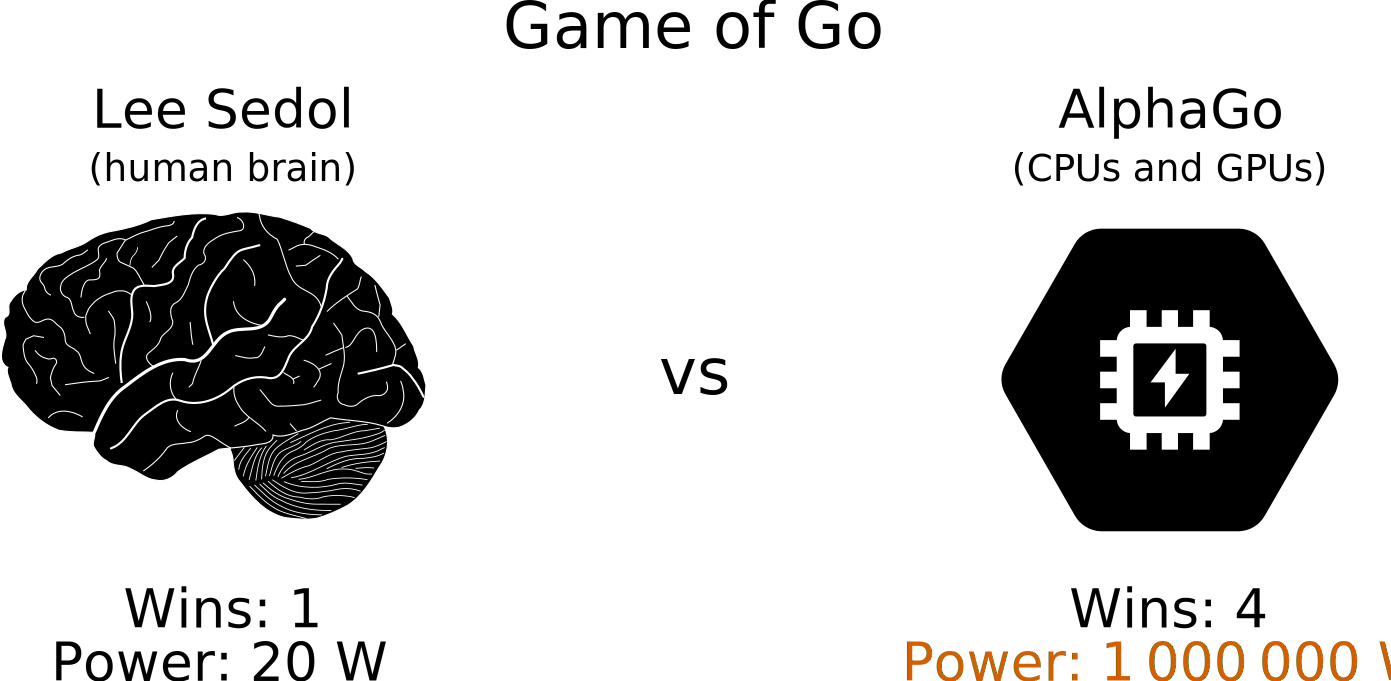
\includegraphics[width=0.7\linewidth]{figures/SVG/brain-vs-computer.pdf}

\end{frame}

\begin{frame}{Context: Emerging Solution}
  \begin{columns}
    \begin{column}{0.45\linewidth}
      \pause{}
      \bigskip

      Neural networks use \ex{vector-matrix products}

      \pause{}
      \bigskip

      \emph{Maybe implement in \ex{hardware}?}

      \pause{}
      \bigskip
      \bigskip

      \concept{Ohm's law} $\rightarrow$ \textcolor{blue}{multiplication}
      \[I_{i, j} = V_i \textcolor{blue}{G_{i, j}}\]

      \pause{}
      \bigskip

      \concept{Kirchhoff's current law} $\rightarrow$ \textcolor{orange}{addition}
      \[I_j = \textcolor{orange}{\sum_i} I_{i, j}\]

    \end{column}

    \pause{}
    \bigskip

    \begin{column}{0.55\linewidth}
      \concept{Crossbar arrays} $\rightarrow$ \ex{vector-matrix products}

      \bigskip

      \resizebox{\linewidth}{!}{%
        \inputtikz{DPE-computation}
      }
    \end{column}
  \end{columns}
\end{frame}

\begin{frame}{Context: Existing Problems}
  \pause{}

  Crossbars may use \concept{memristors}, which
  \pause{}
  \begin{itemize}[<+->]
    \item are \ex{easy to program}
    \item have \ex{good retention}
    \item are \alert{stochastic} and \alert{nonlinear}, especially at high resistance
  \end{itemize}

  \pause[\thebeamerpauses]
  \bigskip

  \centering
  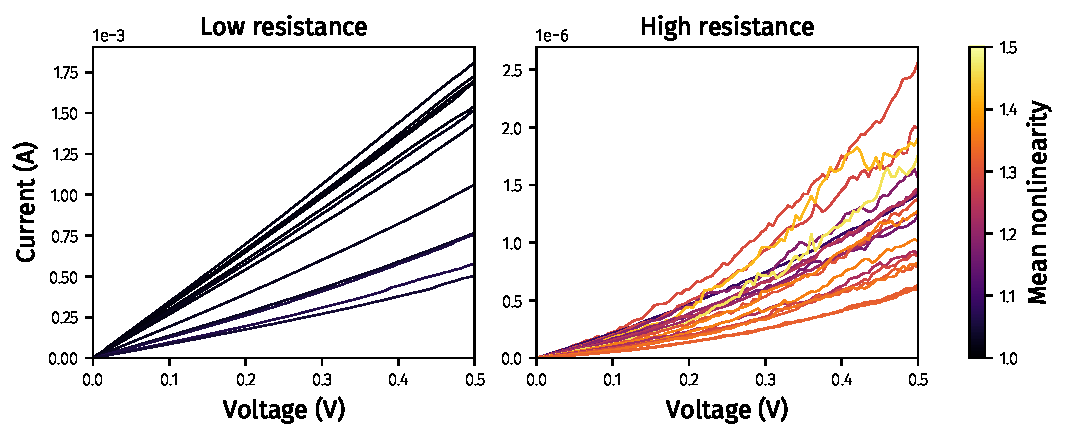
\includegraphics[width=0.8\linewidth]{figures/PDF/SiO_x.pdf}
\end{frame}

\begin{frame}{Solution \#1: Nonlinearity-Aware Training}

  \visible<2->{%
    \begin{columns}
      \begin{column}{0.6\textwidth}
        Typically, input to neuron is
        \[
          \sum_i \alert{x_i w_{i, j}}
        \]
      \end{column}
      \begin{column}{0.4\textwidth}
        \begin{figure}
          \flushleft
          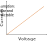
\includegraphics[width=0.6\linewidth]{figures/SVG/linearity-bad.pdf}
        \end{figure}
      \end{column}
    \end{columns}
  }

  \bigskip

  \begin{columns}
    \begin{column}{0.6\textwidth}
      \visible<3->{%
        We propose
        \[
          \sum_i \ex{f}(x_i, w_{i, j})
        \]
        where $\ex{f}$ is nonlinear and stochastic function
      }

      \bigskip

      \visible<4->{%
        Thus, more realistic training
      }
    \end{column}
    \begin{column}{0.4\textwidth}
      \visible<3->{%
        \begin{figure}
          \flushleft
          
\includegraphics[width=0.6\linewidth]{figures/SVG/linearity-good.pdf}
        \end{figure}
      }
    \end{column}
  \end{columns}

\end{frame}

\begin{frame}{Solution \#2: Double Weights}
  \begin{columns}
    \begin{column}{0.75\textwidth}
      \visible<2->{%
        Typically, \alert{one weight mapped onto two conductances}
      }

      \medskip

      \visible<3->{
        Infinite number of possibilities!
        \begin{itemize}
          \item $G_+ = \qty{5}{\milli\siemens} \quad \text{and} \quad G_- = \qty{3}{\milli\siemens}$
          \item $G_+ = \qty{6}{\milli\siemens} \quad \text{and} \quad G_- = \qty{4}{\milli\siemens}$
          \item and so on\ldots
        \end{itemize}
      }
    \end{column}
    \begin{column}{0.25\textwidth}
      \visible<2->{
        \begin{figure}
          \flushleft
          
\includegraphics[width=0.7\linewidth]{figures/SVG/mapping-bad.pdf}
        \end{figure}
      }
    \end{column}
  \end{columns}

  \bigskip
  \bigskip

  \begin{columns}
    \begin{column}{0.75\textwidth}
      \visible<4->{%
        We propose \ex{more direct} relation
      }

      \medskip

      \begin{itemize}
        \item \visible<5->{\emph{training} picks optimal conductances}
        \item \visible<6->{lower conductances through regularisation}
      \end{itemize}
    \end{column}
    \begin{column}{0.25\textwidth}
      \visible<4->{%
        \begin{figure}
          \flushleft
          
\includegraphics[width=0.7\linewidth]{figures/SVG/mapping-good.pdf}
        \end{figure}
      }
    \end{column}
  \end{columns}

\end{frame}

\begin{frame}{Solution \#3: Memristive Validation}

  \begin{columns}
    \begin{column}{0.6\textwidth}
      \visible<2->{%
        Typically, validation error computed \alert{only once} at checkpoints
      }

      \medskip

      \visible<3->{%
        But memristor nonidealities are stochastic!
      }
    \end{column}
    \begin{column}{0.4\textwidth}
      \visible<2->{%
        \begin{figure}
          \flushleft
          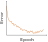
\includegraphics[width=0.6\linewidth]{figures/SVG/validation-bad.pdf}
        \end{figure}
      }
    \end{column}
  \end{columns}

  \bigskip

  \begin{columns}
    \begin{column}{0.6\textwidth}
      \visible<4->{%
        We propose computing validation error \ex{multiple times}
      }

      \medskip

      \visible<5->{%
        \ex{Median} value: better measure of performance
      }
    \end{column}
    \begin{column}{0.4\textwidth}
      \visible<4->{%
        \begin{figure}
          \flushleft
          
\includegraphics[width=0.6\linewidth]{figures/SVG/validation-good.pdf}
        \end{figure}
      }
    \end{column}
  \end{columns}
\end{frame}

\begin{frame}{Results: Training}
  \pause{}

  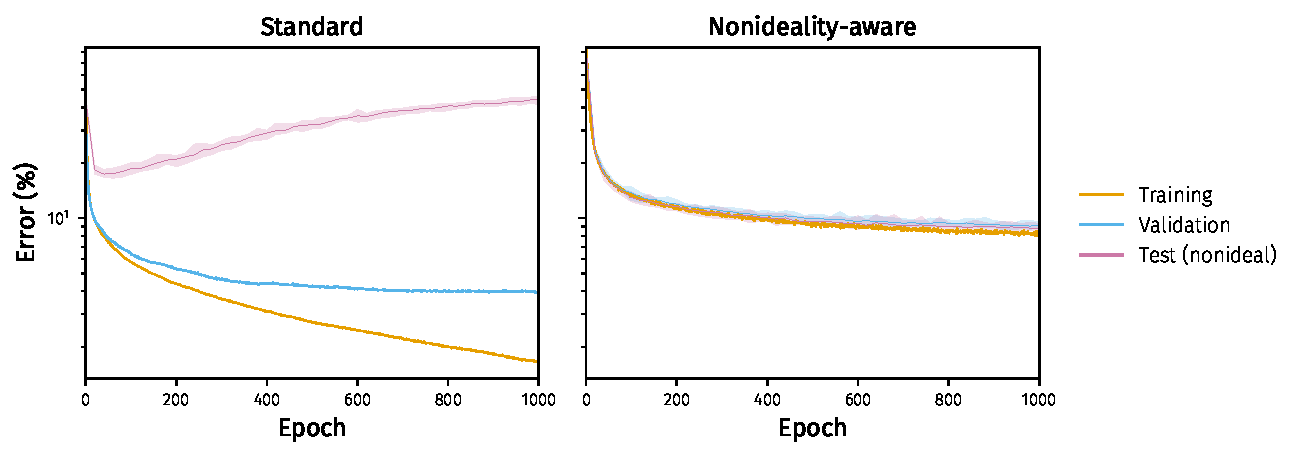
\includegraphics[width=\linewidth]{figures/PDF/iv-nonlinearity-training.pdf}

  \bigskip

  \begin{columns}
    \begin{column}{0.07\textwidth}
    \end{column}
    \begin{column}{0.37\textwidth}
      \pause{}

      Low validation error not indicative of \alert{high test error}
    \end{column}
    \begin{column}{0.37\textwidth}
      \pause{}

      \ex{Lower test error}, similar to validation error
    \end{column}
    \begin{column}{0.19\textwidth}
    \end{column}
  \end{columns}
\end{frame}

\begin{frame}{Results: Inference and Power Consumption}
  \begin{columns}
    \pause{}

    \begin{column}{0.45\linewidth}
      \begin{figure}
        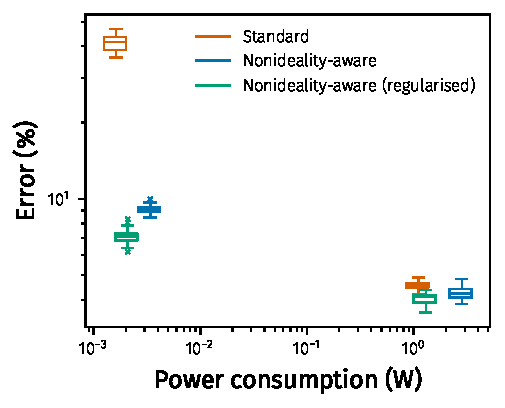
\includegraphics[width=\linewidth]{figures/PDF/iv-nonlinearity-inference.pdf}
      \end{figure}
    \end{column}
    \begin{column}{0.55\linewidth}
      \pause{}

      Low-resistance (right): low error, high power

      \pause{}
      \bigskip

      High-resistance (left) with different training:\pause{}
      \begin{itemize}[<+->]
        \item \alert{standard} $\rightarrow$ high error, low power
        \item \textcolor{blue}{nonideality-aware} $\rightarrow$ lower error
        \item \ex{nonideality-aware + regularised} $\rightarrow$ even lower error and power
      \end{itemize}
    \end{column}
  \end{columns}
\end{frame}

\begin{frame}{Results: Nonideality Agnosticism}
  \begin{columns}
    \begin{column}{0.6\textwidth}
      \pause{}

      \begin{figure}
        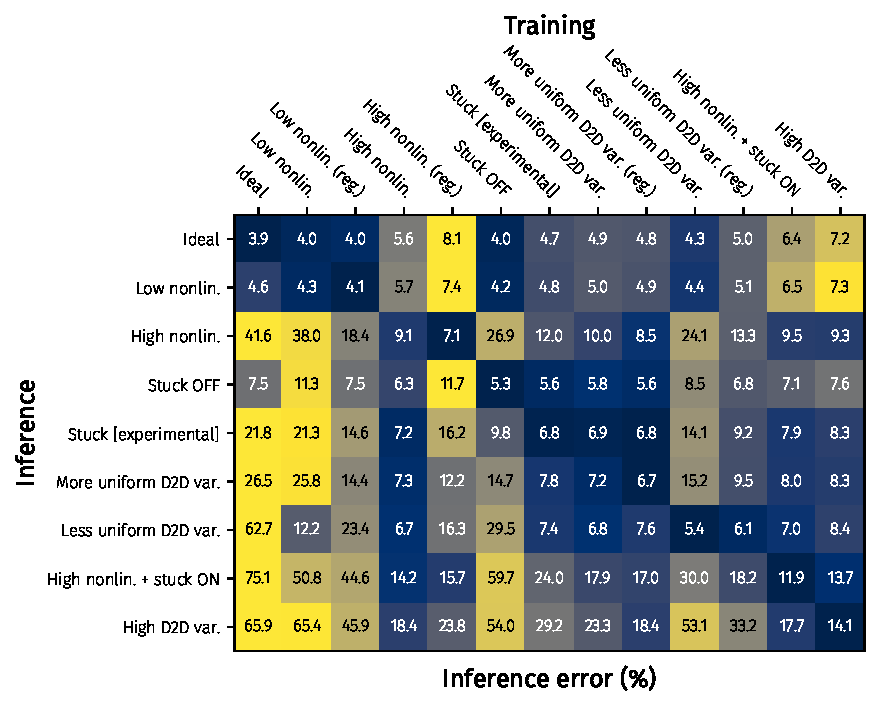
\includegraphics[width=\linewidth]{figures/PDF/nonideality-agnosticism.pdf}
      \end{figure}
    \end{column}
    \begin{column}{0.4\textwidth}
      \pause{}

      Standard training $\rightarrow$ \alert{high error} if nonideal inference

      \pause{}
      \bigskip

      Nonideality-aware training:
      \pause{}
      \begin{itemize}[<+->]
        \item \ex{lower error} if \textbf{expected} nonideality
        \item \ex{lower error} compared to standard (ideal) training if \textbf{unexpected} nonideality
      \end{itemize}
    \end{column}
  \end{columns}
\end{frame}

\begin{frame}{Summary}
  \pause{}

  Solutions to memristor issues:
  \pause{}
  \begin{enumerate}[<+->]
    \item adapt to nonlinearity and stochasticity during training
    \item relate weights to conductances more directly
    \item repeat validation multiple times at checkpoints
  \end{enumerate}

  \bigskip

  \pause[\thebeamerpauses]

  Results:
  \pause{}
  \begin{itemize}[<+->]
    \item training performance \ex{indicative} of inference performance
    \item \ex{lower} test error
    \item \ex{can use} stochastic \& nonlinear high-resistance devices
    \item high \ex{agnosticism} to type of nonideality
  \end{itemize}
\end{frame}

\begin{frame}{Conclusions}
  \pause{}

  Specialised training $\rightarrow$ \ex{accurate} and \ex{robust} memristive neural networks

  \pause{}
  \bigskip

  \ex{No need} to have \emph{perfect} device knowledge

  \pause{}
  \bigskip

  Can afford to use \ex{energy-efficient} high-resistance devices

  \pause{}
  \bigskip

  \ex{Faster adoption} of memristive implementations where low power needed?

\end{frame}

\begin{frame}{The Team}
  \begin{columns}
    \begin{column}{0.6\textwidth}

      \begin{itemize}
        \item \textcolor{gray}{Dovydas~Joksas\textsuperscript{1}}
        \item Erwei~Wang\textsuperscript{2}
        \item Nikolaos~Barmpatsalos\textsuperscript{1}
        \item Wing~H.~Ng\textsuperscript{1}
        \item Anthony~J.~Kenyon\textsuperscript{1}
        \item George~A.~Constantinides\textsuperscript{2}
        \item Adnan~Mehonic\textsuperscript{1}
      \end{itemize}

      \bigskip

      {\footnotesize
        \begin{enumerate}
          \item University College London
          \item Imperial College London
        \end{enumerate}
      }
    \end{column}

    \begin{column}{0.4\textwidth}
      
\includegraphics[width=\linewidth]{figures/PDF/logo-epsrc.pdf}

      \bigskip

      
\includegraphics[width=\linewidth]{figures/PDF/logo-raeng.pdf}
    \end{column}

  \end{columns}
\end{frame}

\begin{frame}{Useful Information}
  \textbf{Paper}\\
  \fullcite{JoWa2022}

  \medskip

  \textbf{Code}\\
  \cleanURL{github.com/joksas/nonideality-aware-mnn-training}

  \medskip

  \textbf{Slides}\\
  \cleanURL{github.com/joksas/emrs-spring-2022}

  \medskip

  \textbf{Email}\\
  \email{dovydas.joksas.15@ucl.ac.uk}\\
  \email{adnan.mehonic.09@ucl.ac.uk}
\end{frame}

\end{document}
